\begin{figure*}[t]
\centering
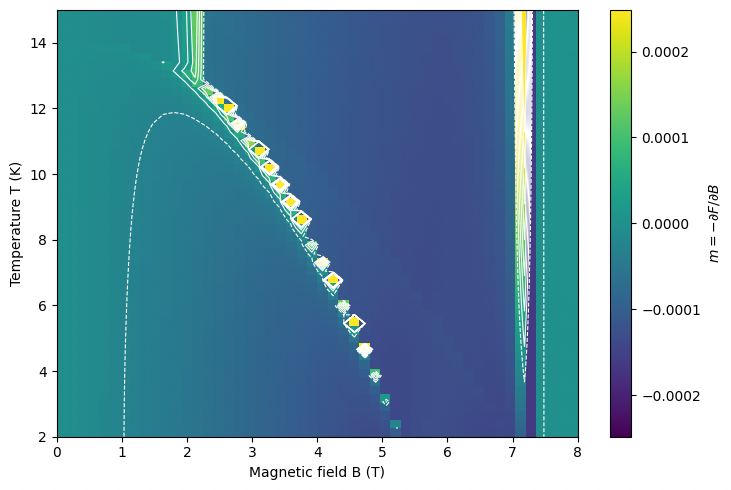
\includegraphics[width=0.48\textwidth]{Figures/CuGeO3-mag.png}
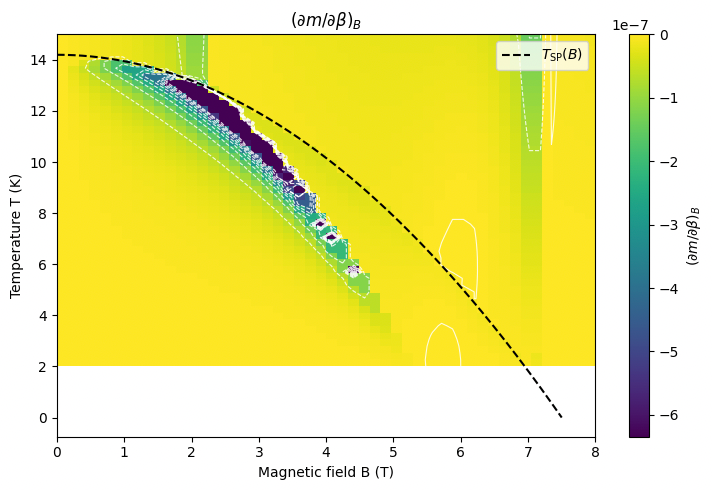
\includegraphics[width=0.48\textwidth]{Figures/CuGeO3-mixed-deriv.png}
\caption{
Response geometry of the spin--Peierls model for \ce{CuGeO3}.
(a) Magnetization landscape \(\langle m\rangle(B,T)\) over the
magnetic-field--temperature control manifold.
(b) Mixed thermal-field response
\((\partial m/\partial \beta)_B\), obtained by differentiating
the free-energy functional. The dashed curve denotes the
spin--Peierls transition scale \(T_{\rm SP}(B)\). The mixed
response develops an extended ridge that tracks the reorganization
of the spin--Peierls state under magnetic field. Unlike the Ising
case, where the response geometry is reconstructed from Monte Carlo
covariances, here the same geometric structure is obtained directly
from a thermodynamic potential.
}
\label{fig:cugeo3_response}
\end{figure*}